\documentclass[11pt,twoside]{article}

\usepackage{amsmath}
\usepackage{amssymb}
\usepackage{amsthm}
\usepackage{courier} % Required for the courier font
\usepackage{extramarks} % Required for headers and footers
\usepackage{fancyhdr} % Required for custom headers
\usepackage{graphicx} % Required to insert images
\usepackage{lastpage} % Required to determine the last page for the footer
\usepackage{listings} % Required for insertion of code
\usepackage{lipsum} % Used for inserting dummy 'Lorem ipsum' text into the template
\usepackage{subcaption}

\usepackage[margin=1in]{geometry}
\usepackage[usenames,dvipsnames]{color} % Required for custom colors

\begin{document}

\title{CSC411 - Project \#2}
\author{Michael Wong - [Student Number]\\Yijin (Catherine) Wang - 998350476}
\maketitle

\clearpage

\section*{Part 1}
\paragraph{Question}
Describe the dataset of digits. In your report, include 10 images of each of the digits. You may find matplotlib’s subplot useful.

\paragraph{Answer}
Please see the images of each digits below. For the same digit, some images have thicker lines (like ``8'' in the second column) and some have thiner lines (like ``8" in the third column). Some digit images are straight (like ``1" in the first column) and some digits are rotated (like ``1" in the ninth column). Most digits are clear to be identified manually but some digits are not clear (like the ``6" in the seventh column). 

\begin{figure*}[h]
	\centering
	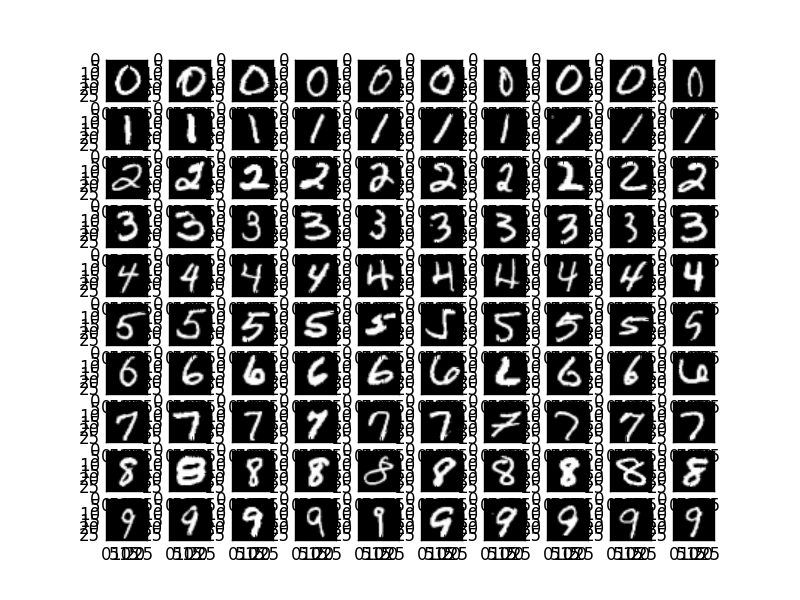
\includegraphics[scale=0.8]{part1.png}
	\caption*{10 images of digits from 0 to 9}
\end{figure*}

\clearpage

\section*{Part 2}

\section*{Part 1}
\paragraph{Question}
Implement a function that computes the network below.
\begin{figure*}[h]
	\centering
	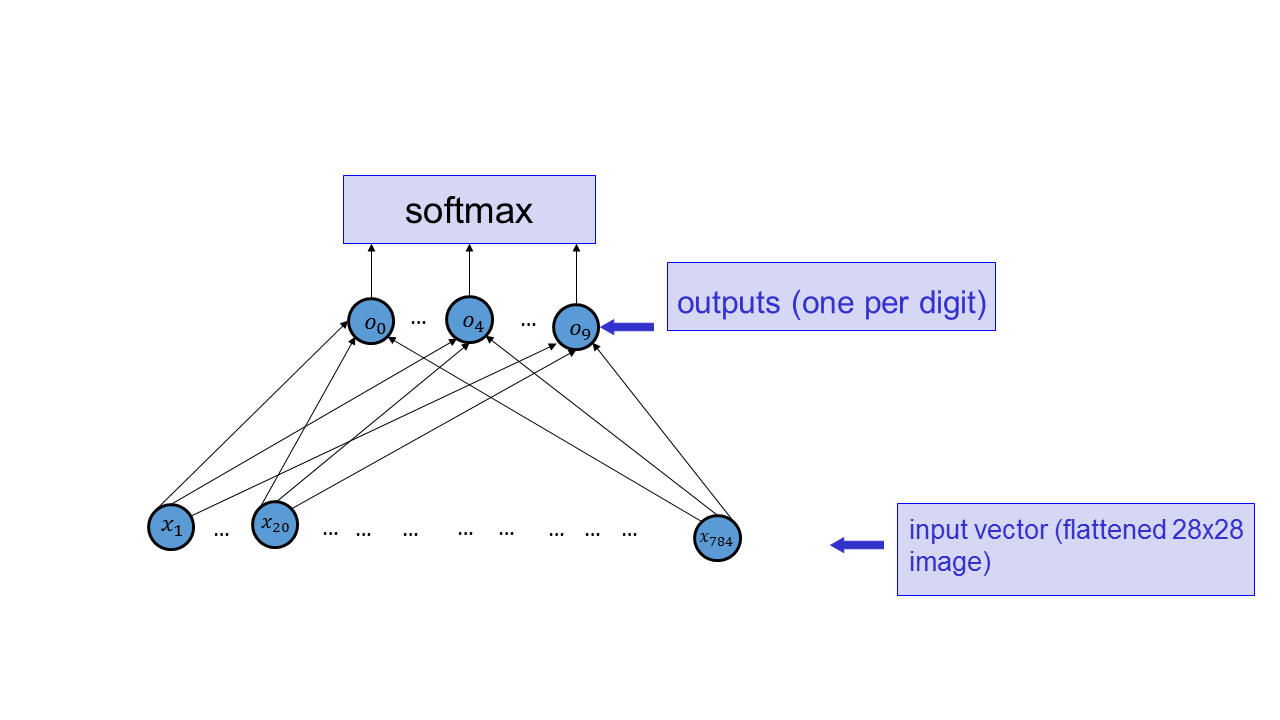
\includegraphics[scale=0.5]{logreg.png}
\end{figure*}
The $o$'s here should simply be linear combinations of the $x$'s (that is, the activation function in the output layer is the identity). Supecifically, use $o_i = \sum_{j}w_{ji}x_j+b_i$. Include the listing of your implementation in your report for this Part.

\paragraph{Answer}
Please see the source code of the function below:

\begin{lstlisting}[language=Python]
def lin_combin_double_layer(W0, W1, b0, b1, x):
    h = lin_combin_single_layer(W0, b0, x)
    return (lin_combin_single_layer(W1, b1, h))
    

def lin_combin_single_layer(W0, b0, x):
    return (dot(W0.T, x) + b0)
\end{lstlisting}
\end{document}